
%% bare_conf.tex
%% V1.3
%% 2007/01/11
%% by Michael Shell
%% See:
%% http://www.michaelshell.org/
%% for current contact information.
%%
%% This is a skeleton file demonstrating the use of IEEEtran.cls
%% (requires IEEEtran.cls version 1.7 or later) with an IEEE conference paper.
%%
%% Support sites:
%% http://www.michaelshell.org/tex/ieeetran/
%% http://www.ctan.org/tex-archive/macros/latex/contrib/IEEEtran/
%% and
%% http://www.ieee.org/

%%*************************************************************************
%% Legal Notice:
%% This code is offered as-is without any warranty either expressed or
%% implied; without even the implied warranty of MERCHANTABILITY or
%% FITNESS FOR A PARTICULAR PURPOSE! 
%% User assumes all risk.
%% In no event shall IEEE or any contributor to this code be liable for
%% any damages or losses, including, but not limited to, incidental,
%% consequential, or any other damages, resulting from the use or misuse
%% of any information contained here.
%%
%% All comments are the opinions of their respective authors and are not
%% necessarily endorsed by the IEEE.
%%
%% This work is distributed under the LaTeX Project Public License (LPPL)
%% ( http://www.latex-project.org/ ) version 1.3, and may be freely used,
%% distributed and modified. A copy of the LPPL, version 1.3, is included
%% in the base LaTeX documentation of all distributions of LaTeX released
%% 2003/12/01 or later.
%% Retain all contribution notices and credits.
%% ** Modified files should be clearly indicated as such, including  **
%% ** renaming them and changing author support contact information. **
%%
%% File list of work: IEEEtran.cls, IEEEtran_HOWTO.pdf, bare_adv.tex,
%%                    bare_conf.tex, bare_jrnl.tex, bare_jrnl_compsoc.tex
%%*************************************************************************

% *** Authors should verify (and, if needed, correct) their LaTeX system  ***
% *** with the testflow diagnostic prior to trusting their LaTeX platform ***
% *** with production work. IEEE's font choices can trigger bugs that do  ***
% *** not appear when using other class files.                            ***
% The testflow support page is at:
% http://www.michaelshell.org/tex/testflow/



% Note that the a4paper option is mainly intended so that authors in
% countries using A4 can easily print to A4 and see how their papers will
% look in print - the typesetting of the document will not typically be
% affected with changes in paper size (but the bottom and side margins will).
% Use the testflow package mentioned above to verify correct handling of
% both paper sizes by the user's LaTeX system.
%
% Also note that the "draftcls" or "draftclsnofoot", not "draft", option
% should be used if it is desired that the figures are to be displayed in
% draft mode.
%
\documentclass[conference]{IEEEtran}
% Add the compsoc option for Computer Society conferences.
%
% If IEEEtran.cls has not been installed into the LaTeX system files,
% manually specify the path to it like:
% \documentclass[conference]{../sty/IEEEtran}





% Some very useful LaTeX packages include:
% (uncomment the ones you want to load)


% *** MISC UTILITY PACKAGES ***
%
%\usepackage{ifpdf}
% Heiko Oberdiek's ifpdf.sty is very useful if you need conditional
% compilation based on whether the output is pdf or dvi.
% usage:
% \ifpdf
%   % pdf code
% \else
%   % dvi code
% \fi
% The latest version of ifpdf.sty can be obtained from:
% http://www.ctan.org/tex-archive/macros/latex/contrib/oberdiek/
% Also, note that IEEEtran.cls V1.7 and later provides a builtin
% \ifCLASSINFOpdf conditional that works the same way.
% When switching from latex to pdflatex and vice-versa, the compiler may
% have to be run twice to clear warning/error messages.






% *** CITATION PACKAGES ***
%
%\usepackage{cite}
% cite.sty was written by Donald Arseneau
% V1.6 and later of IEEEtran pre-defines the format of the cite.sty package
% \cite{} output to follow that of IEEE. Loading the cite package will
% result in citation numbers being automatically sorted and properly
% "compressed/ranged". e.g., [1], [9], [2], [7], [5], [6] without using
% cite.sty will become [1], [2], [5]--[7], [9] using cite.sty. cite.sty's
% \cite will automatically add leading space, if needed. Use cite.sty's
% noadjust option (cite.sty V3.8 and later) if you want to turn this off.
% cite.sty is already installed on most LaTeX systems. Be sure and use
% version 4.0 (2003-05-27) and later if using hyperref.sty. cite.sty does
% not currently provide for hyperlinked citations.
% The latest version can be obtained at:
% http://www.ctan.org/tex-archive/macros/latex/contrib/cite/
% The documentation is contained in the cite.sty file itself.






% *** GRAPHICS RELATED PACKAGES ***
%
\ifCLASSINFOpdf
  \usepackage[pdftex]{graphicx}
  % declare the path(s) where your graphic files are
  % \graphicspath{{../pdf/}{../jpeg/}}
  % and their extensions so you won't have to specify these with
  % every instance of \includegraphics
  % \DeclareGraphicsExtensions{.pdf,.jpeg,.png}
\else
  % or other class option (dvipsone, dvipdf, if not using dvips). graphicx
  % will default to the driver specified in the system graphics.cfg if no
  % driver is specified.
  % \usepackage[dvips]{graphicx}
  % declare the path(s) where your graphic files are
  % \graphicspath{{../eps/}}
  % and their extensions so you won't have to specify these with
  % every instance of \includegraphics
  % \DeclareGraphicsExtensions{.eps}
\fi
% graphicx was written by David Carlisle and Sebastian Rahtz. It is
% required if you want graphics, photos, etc. graphicx.sty is already
% installed on most LaTeX systems. The latest version and documentation can
% be obtained at: 
% http://www.ctan.org/tex-archive/macros/latex/required/graphics/
% Another good source of documentation is "Using Imported Graphics in
% LaTeX2e" by Keith Reckdahl which can be found as epslatex.ps or
% epslatex.pdf at: http://www.ctan.org/tex-archive/info/
%
% latex, and pdflatex in dvi mode, support graphics in encapsulated
% postscript (.eps) format. pdflatex in pdf mode supports graphics
% in .pdf, .jpeg, .png and .mps (metapost) formats. Users should ensure
% that all non-photo figures use a vector format (.eps, .pdf, .mps) and
% not a bitmapped formats (.jpeg, .png). IEEE frowns on bitmapped formats
% which can result in "jaggedy"/blurry rendering of lines and letters as
% well as large increases in file sizes.
%
% You can find documentation about the pdfTeX application at:
% http://www.tug.org/applications/pdftex





% *** MATH PACKAGES ***
%
%\usepackage[cmex10]{amsmath}
% A popular package from the American Mathematical Society that provides
% many useful and powerful commands for dealing with mathematics. If using
% it, be sure to load this package with the cmex10 option to ensure that
% only type 1 fonts will utilized at all point sizes. Without this option,
% it is possible that some math symbols, particularly those within
% footnotes, will be rendered in bitmap form which will result in a
% document that can not be IEEE Xplore compliant!
%
% Also, note that the amsmath package sets \interdisplaylinepenalty to 10000
% thus preventing page breaks from occurring within multiline equations. Use:
%\interdisplaylinepenalty=2500
% after loading amsmath to restore such page breaks as IEEEtran.cls normally
% does. amsmath.sty is already installed on most LaTeX systems. The latest
% version and documentation can be obtained at:
% http://www.ctan.org/tex-archive/macros/latex/required/amslatex/math/





% *** SPECIALIZED LIST PACKAGES ***
%
%\usepackage{algorithmic}
% algorithmic.sty was written by Peter Williams and Rogerio Brito.
% This package provides an algorithmic environment fo describing algorithms.
% You can use the algorithmic environment in-text or within a figure
% environment to provide for a floating algorithm. Do NOT use the algorithm
% floating environment provided by algorithm.sty (by the same authors) or
% algorithm2e.sty (by Christophe Fiorio) as IEEE does not use dedicated
% algorithm float types and packages that provide these will not provide
% correct IEEE style captions. The latest version and documentation of
% algorithmic.sty can be obtained at:
% http://www.ctan.org/tex-archive/macros/latex/contrib/algorithms/
% There is also a support site at:
% http://algorithms.berlios.de/index.html
% Also of interest may be the (relatively newer and more customizable)
% algorithmicx.sty package by Szasz Janos:
% http://www.ctan.org/tex-archive/macros/latex/contrib/algorithmicx/




% *** ALIGNMENT PACKAGES ***
%
%\usepackage{array}
% Frank Mittelbach's and David Carlisle's array.sty patches and improves
% the standard LaTeX2e array and tabular environments to provide better
% appearance and additional user controls. As the default LaTeX2e table
% generation code is lacking to the point of almost being broken with
% respect to the quality of the end results, all users are strongly
% advised to use an enhanced (at the very least that provided by array.sty)
% set of table tools. array.sty is already installed on most systems. The
% latest version and documentation can be obtained at:
% http://www.ctan.org/tex-archive/macros/latex/required/tools/


%\usepackage{mdwmath}
%\usepackage{mdwtab}
% Also highly recommended is Mark Wooding's extremely powerful MDW tools,
% especially mdwmath.sty and mdwtab.sty which are used to format equations
% and tables, respectively. The MDWtools set is already installed on most
% LaTeX systems. The lastest version and documentation is available at:
% http://www.ctan.org/tex-archive/macros/latex/contrib/mdwtools/


% IEEEtran contains the IEEEeqnarray family of commands that can be used to
% generate multiline equations as well as matrices, tables, etc., of high
% quality.


%\usepackage{eqparbox}
% Also of notable interest is Scott Pakin's eqparbox package for creating
% (automatically sized) equal width boxes - aka "natural width parboxes".
% Available at:
% http://www.ctan.org/tex-archive/macros/latex/contrib/eqparbox/





% *** SUBFIGURE PACKAGES ***
%\usepackage[tight,footnotesize]{subfigure}
% subfigure.sty was written by Steven Douglas Cochran. This package makes it
% easy to put subfigures in your figures. e.g., "Figure 1a and 1b". For IEEE
% work, it is a good idea to load it with the tight package option to reduce
% the amount of white space around the subfigures. subfigure.sty is already
% installed on most LaTeX systems. The latest version and documentation can
% be obtained at:
% http://www.ctan.org/tex-archive/obsolete/macros/latex/contrib/subfigure/
% subfigure.sty has been superceeded by subfig.sty.



%\usepackage[caption=false]{caption}
%\usepackage[font=footnotesize]{subfig}
% subfig.sty, also written by Steven Douglas Cochran, is the modern
% replacement for subfigure.sty. However, subfig.sty requires and
% automatically loads Axel Sommerfeldt's caption.sty which will override
% IEEEtran.cls handling of captions and this will result in nonIEEE style
% figure/table captions. To prevent this problem, be sure and preload
% caption.sty with its "caption=false" package option. This is will preserve
% IEEEtran.cls handing of captions. Version 1.3 (2005/06/28) and later 
% (recommended due to many improvements over 1.2) of subfig.sty supports
% the caption=false option directly:
%\usepackage[caption=false,font=footnotesize]{subfig}
%
% The latest version and documentation can be obtained at:
% http://www.ctan.org/tex-archive/macros/latex/contrib/subfig/
% The latest version and documentation of caption.sty can be obtained at:
% http://www.ctan.org/tex-archive/macros/latex/contrib/caption/




% *** FLOAT PACKAGES ***
%
%\usepackage{fixltx2e}
% fixltx2e, the successor to the earlier fix2col.sty, was written by
% Frank Mittelbach and David Carlisle. This package corrects a few problems
% in the LaTeX2e kernel, the most notable of which is that in current
% LaTeX2e releases, the ordering of single and double column floats is not
% guaranteed to be preserved. Thus, an unpatched LaTeX2e can allow a
% single column figure to be placed prior to an earlier double column
% figure. The latest version and documentation can be found at:
% http://www.ctan.org/tex-archive/macros/latex/base/



%\usepackage{stfloats}
% stfloats.sty was written by Sigitas Tolusis. This package gives LaTeX2e
% the ability to do double column floats at the bottom of the page as well
% as the top. (e.g., "\begin{figure*}[!b]" is not normally possible in
% LaTeX2e). It also provides a command:
%\fnbelowfloat
% to enable the placement of footnotes below bottom floats (the standard
% LaTeX2e kernel puts them above bottom floats). This is an invasive package
% which rewrites many portions of the LaTeX2e float routines. It may not work
% with other packages that modify the LaTeX2e float routines. The latest
% version and documentation can be obtained at:
% http://www.ctan.org/tex-archive/macros/latex/contrib/sttools/
% Documentation is contained in the stfloats.sty comments as well as in the
% presfull.pdf file. Do not use the stfloats baselinefloat ability as IEEE
% does not allow \baselineskip to stretch. Authors submitting work to the
% IEEE should note that IEEE rarely uses double column equations and
% that authors should try to avoid such use. Do not be tempted to use the
% cuted.sty or midfloat.sty packages (also by Sigitas Tolusis) as IEEE does
% not format its papers in such ways.





% *** PDF, URL AND HYPERLINK PACKAGES ***
%
%\usepackage{url}
% url.sty was written by Donald Arseneau. It provides better support for
% handling and breaking URLs. url.sty is already installed on most LaTeX
% systems. The latest version can be obtained at:
% http://www.ctan.org/tex-archive/macros/latex/contrib/misc/
% Read the url.sty source comments for usage information. Basically,
% \url{my_url_here}.





% *** Do not adjust lengths that control margins, column widths, etc. ***
% *** Do not use packages that alter fonts (such as pslatex).         ***
% There should be no need to do such things with IEEEtran.cls V1.6 and later.
% (Unless specifically asked to do so by the journal or conference you plan
% to submit to, of course. )


% correct bad hyphenation here
\hyphenation{op-tical net-works semi-conduc-tor}


\begin{document}
%
% paper title
% can use linebreaks \\ within to get better formatting as desired
\title{Multiple Instance Learning of Clinical Phenotype Based on Metagenome-Wide Association Study}

% affiliations
\author{\IEEEauthorblockN{Nathan LaPierre}
\IEEEauthorblockA{Department of Computer Science\\
George Mason University\\
Fairfax, Virginia 22030\\
Email: nlapier2@masonlive.gmu.edu}
\and
\IEEEauthorblockN{Mohammad Rahman}
\IEEEauthorblockA{Department of Computer Science\\
George Mason University\\
Fairfax, Virginia 22030\\
Email: arif.at.iut@gmail.com}
\and
\IEEEauthorblockN{Huzefa Rangwala}
\IEEEauthorblockA{Department of Computer Science\\
George Mason University\\
Fairfax, Virginia 22030\\
Email: rangwala@cs.gmu.edu}
}

% conference papers do not typically use \thanks and this command
% is locked out in conference mode. If really needed, such as for
% the acknowledgment of grants, issue a \IEEEoverridecommandlockouts
% after \documentclass

% for over three affiliations, or if they all won't fit within the width
% of the page, use this alternative format:
% 
%\author{\IEEEauthorblockN{Michael Shell\IEEEauthorrefmark{1},
%Homer Simpson\IEEEauthorrefmark{2},
%James Kirk\IEEEauthorrefmark{3}, 
%Montgomery Scott\IEEEauthorrefmark{3} and
%Eldon Tyrell\IEEEauthorrefmark{4}}
%\IEEEauthorblockA{\IEEEauthorrefmark{1}School of Electrical and Computer Engineering\\
%Georgia Institute of Technology,
%Atlanta, Georgia 30332--0250\\ Email: see http://www.michaelshell.org/contact.html}
%\IEEEauthorblockA{\IEEEauthorrefmark{2}Twentieth Century Fox, Springfield, USA\\
%Email: homer@thesimpsons.com}
%\IEEEauthorblockA{\IEEEauthorrefmark{3}Starfleet Academy, San Francisco, California 96678-2391\\
%Telephone: (800) 555--1212, Fax: (888) 555--1212}
%\IEEEauthorblockA{\IEEEauthorrefmark{4}Tyrell Inc., 123 Replicant Street, Los Angeles, California 90210--4321}}




% use for special paper notices
%\IEEEspecialpapernotice{(Invited Paper)}




% make the title area
\maketitle


\begin{abstract}
%\boldmath
%abs

We demonstrate a computational method to predict the clinical
phenotypes of a patient from raw metagenomic sequence read data. We  compared 
two state of the art programs for annotating the sequence data, 
UCLUST and Kraken, and using their output for feature generation. 
We apply these programs 
to a set of over 1.3 million reads from 
904 patients, some of whom have liver cirrhosis, encephalopathy due to liver cirrhosis, or 
neither disease. Once the reads have been processed by UCLUST or 
Kraken, we use  Support Vector Machines to setup the 
clinical phenotype prediction problem.  
%
We find that too many false negatives are being predicted by 
the classifier. In order to address the issue, we scale features to
improve the classification model and evaluate the 
end results on a held-out test set. We
demonstrate our approach works quickly and 
accurately with an 85.64\% success rate when we use the 
UCLUST representation. We also find that UCLUST generally performs better than Kraken, with the latter having an 80.66\% success rate. We also test our classifier on several subsets of the data, with success rates ranging from 69.81\% to 96.72\%.


\end{abstract}
% IEEEtran.cls defaults to using nonbold math in the Abstract.
% This preserves the distinction between vectors and scalars. However,
% if the conference you are submitting to favors bold math in the abstract,
% then you can use LaTeX's standard command \boldmath at the very start
% of the abstract to achieve this. Many IEEE journals/conferences frown on
% math in the abstract anyway.

% no keywords




% For peer review papers, you can put extra information on the cover
% page as needed:
% \ifCLASSOPTIONpeerreview
% \begin{center} \bfseries EDICS Category: 3-BBND \end{center}
% \fi
%
% For peerreview papers, this IEEEtran command inserts a page break and
% creates the second title. It will be ignored for other modes.
\IEEEpeerreviewmaketitle



\section{Introduction}

%Intro

The human body contains one of the most dense and diverse microbial environments in the world. The human and microbial cells are collectively referred to as the \emph{human microbiome} \cite{turnbaugh_human_2007,backhed_host-bacterial_2005}. Advances in biotechnology have allowed scientists to directly interrogate the human microbiome, particularly the development of high throughput sequencing technologies, which generate massive amounts of biological data. In recent years, improving capabilities in data science have allowed for the study of \emph{metagenomics}, which involves sequencing the entire pool of microbial genomes at once. This data is usually gathered via \emph{shotgun sequencing}, which generates a number of short \emph{reads} containing bits of genomic data from the microbes of the host environment \cite{messing81}. These reads, represented as strings of nucleotides, represent only small parts of the microbe's full genome, and are not ordered in any way, which presents several challenges that will be discussed further in the paper. 

Metagenomics has several advantages: (i) microbes are now understood to be the underlying cause of many human diseases and are also critical to many chemical processes and overall health; (ii) it is believed that most microbes have not been laboratory-cultured and thus remain unknown; (iii) whereas other methods such as 16S rRNA analysis are mainly useful for predicting the species of microbes (\emph{phylogeny}), metagenomics contains other critical information from the microbial genomes that determine how these microbes function and affect diseases and chemical processes (\emph{functional} information) \cite{handelsman04}. Summarily, metagenomics allows us to view microbial data that is not accessible to us via traditional laboratory culturing and allows for both phylogenetic and functional profiling of those microbes. Thus, studying microbial metagenomics is an effective way to predict and model human disease, also known as clinical \emph{phenotype}.

In this study, we develop an efficient classifier that predicts whether or not a patient has a disease based on their microbiome. This can be viewed as a Multiple Instance Learning (MIL) problem, in which we have several \emph{bags} of instances, and we have labels for the bags, but not for each instance within them. In this case, we have a patient (bag) and a label for each patient (whether or not they have a disease), but no labels for each patient's sequence reads (instances). Specifically, we use a Distance-based Bag of Words (D-BoW) method, discussed further in the Background section, which has been shown to be among the most effective and efficient MIL methods \cite{amores13}. We also show that our pipeline can be used for Histogram-based Bag of Words (H-BoW) methods. MIL has been studied in many contexts, but it has rarely if ever been studied in the context of predicting clinical phenotype based on metagenomic data from the microbiome. However, since datasets in this domain frequently have patient-level labels but almost never have instance-level labels, this is a well-suited domain for multiple instance learning. 

We used data from a Metagenome-Wide Association Study (MGWAS), which compares microbial metagenomic data between many patients with or without a given phenotype. Because MGWAS studies contain many expert-labeled patients and the metagenomic data associated with those patients, they are very useful for phenotype prediction but also cause many computational challenges. The data is very large (multiple terabytes) and high-dimensional (thousands of dimensions). Additionally, due to the nature of shotgun sequencing, most of the reads are not useful by themselves, and must first be assembled. \emph{Assembly} is the process of finding pairs of reads in which the end of one read overlaps with the beginning of another, signifying that they are probably contiguous reads from the same genome, and combining them. This process is repeated as much as possible to form long strings called \emph{contigs}. Assembly also reduces the size and dimensionality of the data by discarding reads that cannot be assembled successfully. Most of the discarded reads would not be particularly useful anyway, since the assembly process could not establish their relationship to other reads and many of them are due to sequencing machine errors. The reduction in data size also allows for clustering, which is not feasible for massive datasets. Clustering uses string similarity measures to group similar reads into "clusters", which is a way of identifying which species of microbe each read corresponds to. The alternative, "aligning" the reads with known genomes, is both time-inefficient and impractical for metagenomics, since many of the involved microbes have not yet had their genomes sequenced. From the clustering output, we extract feature vectors, which are then fed into a standard Support Vector Machine (SVM) classifier. 

Thus, the entire pipeline consists of assembling the reads of each patient, combining the resulting contigs from each patient into a single file, clustering the contigs, extracting features from the clustering output, and performing classification with the SVM. This process is explained in further detail in the methods section. We refer to the pipeline as "CAMIL", which stands for Clustering and Assembly with Multiple Instance Learning. We then compare the results of our classifier against the classifier used in the MGWAS study from which we derived our data. We show that our classifier shows significantly improved performance. This is discussed further in the Experimental Results section.

The rest of the paper is organized as follows. Section 2 presents relevant Background information on  Multiple Instance Learning, Assembly, and Clustering. Section 3 presents the Methods we used in the creation of our pipeline. Section 4 presents Materials, such as dataset, hardware, and software descriptions. Section 5 presents our Results, and Section 6 presents our Conclusions.


\section{Background}
%RELATED

\subsection{Multiple Instance Learning}

The Multiple Instance Learning (MIL) problem was first described by Dietterich in the context of drug activity prediction \cite{dietterich97}. In this problem, we want to figure out which of a number of different molecules will bind to a target "binding site". Each molecule can assume a number of different 3-dimensional shapes, so even for molecules that are known to bind to the binding site, it is not necessarily known which formation of the molecule succeeds in binding. If even one shape of a given molecule binds to the binding site, it is considered a "good" molecule \cite{dietterich97}. Thus, in the original formation of MIL, a bag is classified as positive if one or more instances within it is positive, while a negative bag contains all negative instances. In the original paper, Dietterich develops a solution based on axis-parallel rectangles to solve this problem, and the MIL approach was shown to be significantly more effective than a standard supervised learning approach \cite{dietterich97}. In the late 1990s and early 2000s, a number of different approaches were developed for the original MIL problem, such as Diverse Density (DD) \cite{perez98}, EM-DD \cite{zhang01}, MI-SVM \cite{andrews02}, sbMIL \cite{bunescu07}, and MILES \cite{wang06}. A recent review of MIL by Amores created a taxonomy of these various methods and compared their effectiveness for classification \cite{amores13}.
%

However, since 2010, there has been increased interest in different formulations of the MIL problem. For instance, the problem of "key instance detection" \cite{zhou12} revolves around finding the instances that contribute the most to bag labels. A recent study focused on a formulation of the MIL problem in which bags with negative labels can contain some "positive" instances, and developed a general cost function for determining individual instance labels from group labels \cite{kotzias15}. This is significant in metagenomics because, while some diseases are caused by a single pathogen, many arise from a combination of many factors, and even patients that are "healthy" may contain small amounts of pathogens that are normally associated with disease. 
%

However, this method treats a group label simply as an aggregation of instance labels. Amores, in his taxonomy, called this type of method "Instance-based", and found this paradigm to be ineffective \cite{amores13}. Amores identifies two other paradigms, Bag-Space and Embedded-Space. An example of the latter are Bag of Words (BoW) methods, which involve the following three-step process: (i) Cluster the instances to create classes of instances; (ii) for each bag, map the clusters of instances in that bag to a feature vector; and (iii) use a standard classifier that uses the feature vectors to predict group labels \cite{amores13}. Amores found the Distance-based Bag of Words (D-BoW) method to be the second most effective of all tested methods, and the most effective one that was also time-efficient \cite{amores13}. The distinguishing feature in D-BoW methods is that the values for the feature vector represent the instance that has the smallest distance to the cluster center. Despite these recent developments in MIL, we have not found any literature that specifically applies MIL to classifying patient phenotype based on metagenomic data.

\subsection{Assembly}

\begin{figure}[h]
\centering
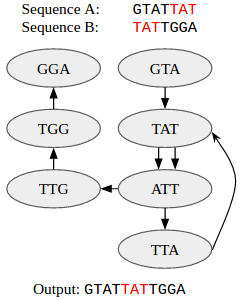
\includegraphics[scale=0.5]{./de-bruijn.png}
\caption{This diagram illustrates a basic de Bruijn graph, as explained in the text. Notice the double arrow from TAT to ATT, allowing a path to go through that route twice. Thus, the longest contig that can be created by following a path is GTATTATTGGA, which is what we want.} \label{de-bruijn}
\end{figure}

The \emph{assembly} problem involves combining overlapping short reads (usually less than 1000 base pairs) into longer sequences called \emph{contigs} (often tens of thousands of base pairs). For instance, if one read ends with the same relatively large nucleotide string that another read starts with, the reads are likely to be overlapping fragments from the same genome, and can thus be combined into one contig. This can be done either \emph{de novo} (in an unsupervised manner) or by referencing sequences against known contigs. We focus on de novo assembly, because we wish to keep our pipeline as unsupervised as possible. 

One of the main purposes of assembly is to determine the whole genomes of microbial species, the vast majority of which have not or cannot be laboratory cultured, from sequencing reads \cite{zerbino08}. Even if full genomes cannot be assembled, combining reads into larger contigs can still make them much more useful for clustering and classifiers, because the contigs will contain more phylogenetic and functional information than short reads. This is because short reads of less than 1000 base pairs constitute only a tiny fraction of microbial genomes, which are usually hundreds of thousands to millions of base pairs, making it difficult to ascertain much about the phylogeny of individual reads. Many modern sequence reads are produced by Next-Generation and High-Throughput Sequencers, which usually produce these short reads. Metagenomics additionally poses its own set of challenges, due to very large datasets and lack of knowledge about how many species are present and in what relative abundances \cite{namiki12}. Thus, metagenome assembly is a relatively new and challenging field.

Some of the popular genome and metagenome assembly approaches include SOAPdenovo2 \cite{luo12}, IDBA-UD \cite{peng12}, Velvet \cite{zerbino08}, MetaVelvet \cite{namiki12}, ABySS \cite{simpson09}, and Ray Meta \cite{boisvert12}. We used SOAPdenovo2 in our study, because it was the assembler used in the original MGWAS study \cite{qin041012} and because it has been shown to be one of the fastest assembly algorithms \cite{peng12}. SOAPdenovo2 first constructs a type of directed graph called a \emph{de Bruijn} graph that represents the overlaps between different sequences \cite{li10}. Reads are divided into strings of length K called \emph{k-mers}; these k-mers are the nodes of the graph \cite{zerbino08}. The choice of K is up to the user, and is important for having good assembly results. The k-mer nodes in the graph have an edge between them if a read contains those k-mers in order with an overlap of K-1 nucleotides, and the direction of the edge indicates in which order the k-mers appear \cite{zerbino08}. SOAPdenovo2 then cleans this graph by removing nodes/sequences with few or no connections with other sequences, eliminating "tips" that represent likely sequencing machine errors, and removing redundant edges \cite{li10}. The contigs are then formed by combining reads according to the de Bruijn graph: each contig represents a directed path in the graph \cite{zerbino08}. There are variations on how exactly de Bruijn graphs are represented and implemented, but Figure \ref{de-bruijn} illustrates the general process.

\subsection{Clustering}

\begin{figure}[h]
\centering
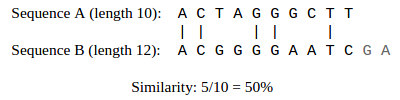
\includegraphics[scale=0.5]{./uclust-similarity.png}
\caption{This diagram illustrates the similarity computation between two sequences in UCLUST. Terminal characters are excluded, so the length of the reads is 10. In the first 10 characters of each string, there are 5 matching characters that are in the same position in the string. Thus, the similarity is 5/10 = 50\%.} \label{uclust-similarity}
\end{figure}

The \emph{clustering} problem in this context  involves grouping input short reads  such that reads within a group are similar to each other. The clusters obtained from this process are referred to as Operational Taxonomic Units (OTUs). OTUs represent a group of equivalent or similar organisms. Accordingly, the number of OTUs in a sample gives an approximation of the species diversity in that sample  \cite{schloss2009introducing,schloss2005introducing,sun2009esprit}.
In addition to approximating species diversity, clustering has several other key advantages. Because clustering is always de novo (unsupervised), it is not limited by the species that are covered in taxonomic databases. This detail is important, because it is believed that most microorganisms that reside in the human body have not been laboratory cultured \cite{handelsman04}. Clustering also reduces computational costs by allowing analyses to operate on entire clusters instead of on each read. Finally, clustering helps the classification process by allowing feature vectors to be built at the OTU level, instead of using individual short reads that contain little biological information.

UCLUST \cite{Edgar10}, CD-HIT \cite{Li01072006}, mothur \cite{schloss2009introducing}, DOTUR \cite{schloss2005introducing}, CROP \cite{Hao01032011}, MC-MinH \cite{sdm2013a}, and 
MC-LSH \cite{bibm2012} are some of the popular  nucleotide sequence clustering approaches. We use UCLUST within our study, which is one of the most widely used and cited metagenome clustering methods and has been shown to be amongst the most effective in terms of speed and accuracy in benchmarking studies \cite{bonder090112, sun042711}. 
%

UCLUST seeks to ensure that, for some similarity T, the following conditions hold: (i) all cluster centroids have a similarity of less than T to each other; and (ii) all points in a cluster have a similarity of greater than T to the cluster centroid \cite{Edgar10}. Thus, each \emph{centroid} defines the center of a cluster, and the distance T defines the radius of the cluster, such that any point that has a similarity of greater than T to the centroid is within the radius and is thus part of the cluster. UCLUST is a heuristic algorithm that has several optimizations to improve speed, thus condition (i) above is not always guaranteed \cite{Edgar10}. UCLUST proceeds in a greedy, iterative manner. The first sequence in the input file becomes a new cluster centroid. For each new sequence in the file, it is compared with each of the existing cluster centroids in order. As soon as it is compared with a centroid that it has a similarity of greater than T with, it becomes part of that cluster. If the read is not similar enough with any of the existing cluster centroids, it becomes the centroid of a new cluster. The similarity measure T is defined as a string similarity between the two nucleotide sequences that counts the number of character placements that they have in common and then divides that number by the length of the reads, with terminal characters excluded \cite{Edgar10}. This is illustrated in figure \ref{uclust-similarity}.

\section{Methods}
%methods

\subsection{Overview}

Figure \ref{fig1} provides an overview of the 
developed computational pipeline. 
%
We obtain 16S metagenomic sequence reads from patients who 
had encephalopathy and liver cirrhosis, no encephalopathy but liver cirrhosis, and controls (with neither phenotype). The input sequence 
reads are annotated using a taxonomic profiling approach (Kraken) or 
an unsupervised binning approach (UCLUST). The output of this annotation phase 
features are generated, which are passed on the binary support vector machine 
classifier (SVMs).  We used the  svm-light implementation \cite{Joachims08}  
to perform the classification of whether or not a patient 
had a clinical phenotype. We compared the classification performance of the 
SVM classifier with the two intermediate sequence representations obtained from 
UCLUST and Kraken. We also applied feature scaling and 
selection techniques to improve the classification results.

\begin{figure*}[t]
\begin{center}
\caption{Pipeline Overview. \label{fig1}}
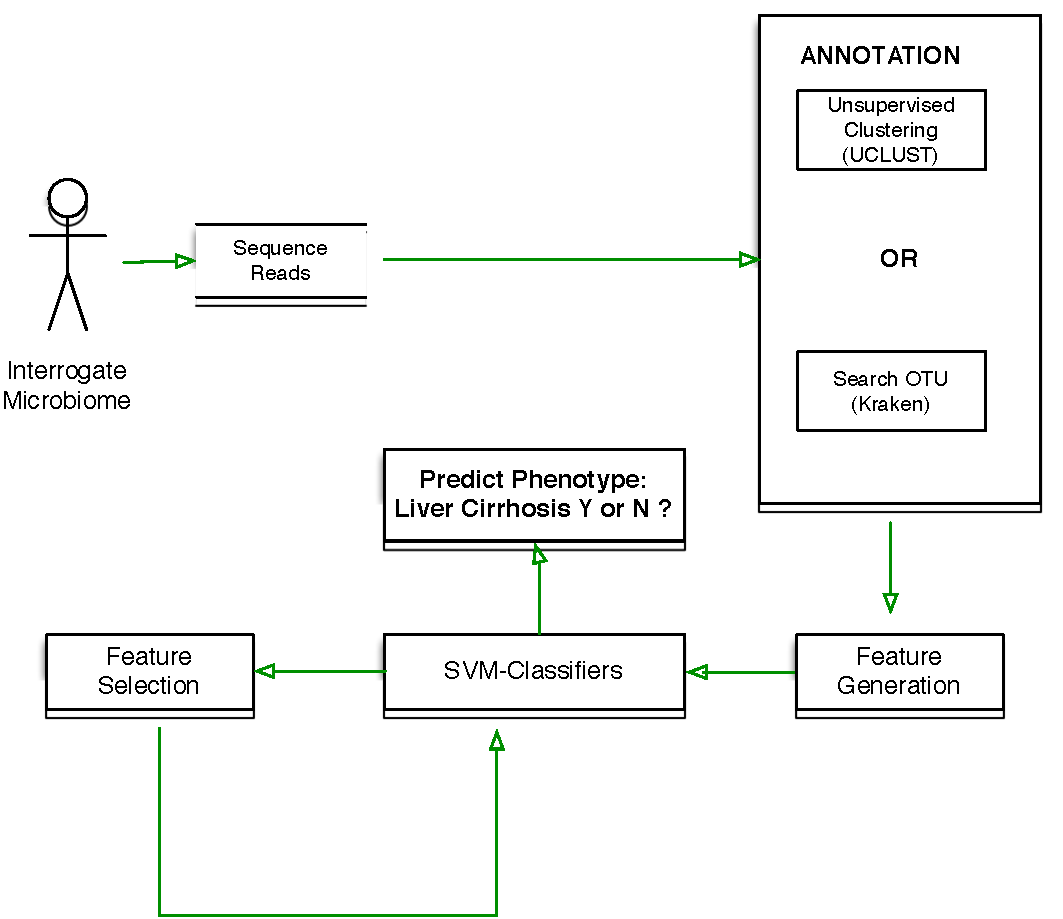
\includegraphics[scale=0.7]{./diagrams/concept}
\end{center}
\end{figure*}

\subsection{Unsupervised Clustering using UCLUST}
\label{uclustmethods}

In this work we evaluate the use of an unsupervised approach 
for representing our input metagenome sequence reads. Specifically, we 
  use UCLUST \cite{edgar2010search} due to its superior performance in terms 
  of run time and accuracy.
%
%
%
UCLUST \cite{edgar2010search} follows a greedy, iterative clustering approach. As a first 
step, this approach identifies exact matches of fixed length between sequence pairs known 
as seeds. These seeds are then extended by allowing for a few mismatches and/or gaps between 
the aligned pairs. Seeds scoring above a certain threshold are chosen as high segment pairs (HSPs)  and 
used for further processing. As such, the step eliminates a lot of pairwise comparisons. 

Then UCLUST follows an 
incremental approach for assigning the input sequences to the different bins. 
%
%
The clustering solution is initialized as an empty list. Sequences are then 
incrementally added to the clusters existing within the list. 
%
Each unassigned input sequence is compared to the cluster representatives within the list using 
the fast indexing search technique that uses the HSPs. If a match is found with one of the 
cluster representatives, then that sequence is assigned to that particular cluster or the 
input sequence forms a new cluster. 
%
UCLUST ensures
that the cluster representatives are sequences with the largest length. 

\subsection{Supervised Taxonomic Identification using Kraken}

We also evaluate the use of a search based 
approach to taxonomically label our sequence reads. We use 
Kraken for this, due to its strong performance in terms of run time 
and precision. Kraken finds $k$-mers in an input 
sequence read and queries a database of OTUs. It then associates the 
read with the lowest common ancestor (LCA) of the genomes that contains $k$-mers from the read \cite{Kraken}. In order to reduce 
the number of false positives, Kraken does not classify reads for 
which it does not find sufficient evidence of any match.


This approach is designed to perform quickly and with 
high precision. However, it also involves downloading and building 
a large database to query. It is often infeasible to download and 
build the database in its entirety, so a smaller custom  
subset of the database is available for testing 
purposes. We used this 
subset of the entire database in this study (referred to as kraken-light).


\subsection{Classification using Support Vector Machines (SVMs)}

Support Vector Machines (SVMs) \cite{vap95} are 
one of the most powerful and versatile binary classifiers used 
in myriad applications. 
%
For a  binary classification problem, the support 
vector machine (SVM) \cite{vap95} framework 
maximizes the separation between the two classes.
%

Given an input set of positive training instances and 
negative training instances, the SVM classifier learns a 
mathematical function $f$  that maximizes the separation between 
the given positive and negative training instances. The function $f$ will then be able to predict whether a new instance (considered a test instance) should have a positive or negative class label.
%
For our formulation we use SVMs to make clinical phenotype prediction for each 
patient sample 
based on their  input metagenome sequence samples represented with their 
clustering or taxa membership features. 

For all the available microbiome samples,  we have a set of reads processed via UCLUST or Kraken. 
%
Each patient is associated with a vector that is used by the SVM to help build $f$. Each row in the vector, called a feature, corresponds to a certain species, and the value for that row corresponds to how closely the read from the patient matched what the species was expected to look like. The exact process of assembling a feature vector for a 
patient depends on which data representation is being used. For 
UCLUST, we use each cluster seed 
as a feature. For each input 
sequence, we use the percentage match to its cluster seed as 
the value for that feature and average the 
sequence match if multiple reads from the metagenome samples 
are assigned to the same cluster by UCLUST. 
%
For Kraken, we use the taxonomic label associated 
with the read as the feature for the SVM. The percentage match of the 
read to that label is used as the feature value. Similar 
to UCLUST, we average the similarity score if multiple reads align to the 
same taxonomic class label. 
%
Our feature selection process involves discarding Kraken's unlabeled 
reads and UCLUST's clusters with only one read (singletons). 

We used cross-validation and a held out set procedure (discussed in the next 
Section) to assess the performance of SVM classification using UCLUST and Kraken
as intermediate representations.




\section{Materials}
\subsection{Dataset Description}

We obtained 904
clinical microbiome samples from a study by Dr. Patrick Gillevet 
that relates to patients who suffered from hepatic encephalopathy due 
to liver cirrhosis. Specifically, the classification formulation 
was setup to distinguish between patients suffering with a specific 
clinical phenotype or not. There were a total of 239 
patients with Encephalopathy   due to liver cirrhosis (denoted 
by the ``Encephalopathy'' class), 590 patients with liver cirrhosis 
but no Encephalopathy (denoted by ``No Encephalopathy'') 
and 75 patients who were considered as 
control and did not have either of the clinical conditions (denoted by ``Control'').
%
16S rRNA metagenomic sequence read data was 
obtained from patient stool samples. On average 
there were a total of 1,464  sequence reads of length 200-400 obtained per 
patient, with 1,323,016 total reads across all patients in our dataset.



\subsection{Evaluation Metrics}
We assess the performance of our classification pipeline 
in terms of correctness and execution time.
%
Given the imbalanced nature of class distributions,  the 
performance of  binary classifiers was measured by 
F1 score, precision and recall, along with
the standard accuracy metric. We discuss 
these standard metrics in brief.

Accuracy measures the percentage of instances 
that are classified correctly and can 
be represented by 
\begin{equation}
Accuracy = (TP + TN)/ (TP + TN + FP + FN)  \label{eqn:acc} 
\end{equation}
where TP, TN, FP and FN represents true positives, true negatives, false positives and false negatives respectively.

Accuracy as an evaluation metric can be biased if one of the classes 
(positive or negative)  has a larger number of examples than the other.   
Precision measures the percentage of positive predictions that 
were correct, 
whereas recall measures the percentage of positive 
examples that were correctly predicted (or retrieved). 
We can represent Precision and Recall by \cite{Goutte}:

\begin{equation}
Precision = TP / (TP + FP). \label{eqn:prec}
\end{equation}
\begin{equation}
Recall = TP / (TP +FN). \label{eqn:roc}
\end{equation}

The F1 score captures the trade offs between precision and recall in a
single metric and is the harmonic mean of precision and recall \cite{Goutte}, given 
by:
\begin{equation}
F1-Score = 2 * (Precision * Recall)/ (Precision + Recall). \label{eqn:f1}
\end{equation}

\subsection{Software and Hardware Details}
We used the Argo computing cluster available at George Mason University. 
%
The representation generation phase using UCLUST and Kraken and and the classification phase
were 
run on one of the  compute nodes available on the cluster. The cluster is configured with 
35 Dell C8220 Compute Nodes, each with dual 
Intel Xeon E5-2670 (2.60GHz) 8 core CPUs, with 64 GB RAM. (Total Cores – 
528 and 1056 total threads, RAM \textgreater 2TB)\cite{ORC}.

Source codes for UCLUST \cite{Edgar10} and KRAKEN \cite{Wood14} were downloaded from 
their respective websites\footnote{UCLUST: http://www.drive5.com/uclust/downloads1\_{}2\_{}22q.html     
Kraken: https://ccb.jhu.edu/software/kraken/} and compiled on the Argo platform. 
%
Kraken aligns reads to an OTU database. The standard Kraken database is 160GB in size. Due to 
computational limitations we used the custom, small sized 4GB
database  in this feasibility study \cite{Kraken}.

For the  SVM-based classification\cite{Joachims08}  we used the popular 
SVM-Light \cite{Joachims08}  source code, which is publicly 
available \footnote{http://svmlight.joachims.org/}.  The linear kernel was used
and the regularization parameters were set to their default values. 



\subsection{Experimental Protocol}

For evaluating the performance of our binary phenotypic classifiers, we 
split the patient samples into a training set containing 80\% of the 
patients and the test set containing 20\% of the patient samples. Every fifth sample was placed in the test set, so the relative class sizes were roughly consistent between the training and test sets.
We also performed leave-one-out cross validation (LOOCV). 

In the next section, we discuss the accuracy of our 
classifier with regards to predicting the clinical 
phenotype of a given patient using 
either the unsupervised 
clustering representation with UCLUST or 
supervised OTU representation 
with Kraken. We present results for classifiers 
distinguishing patients  in the ``Encephalopathy'' class versus
the other classes, effectively 
determining whether or not a patient had Encephalopathy 
regardless of whether they had liver cirrhosis. We also 
present pairwise one-versus-one classification results that 
compared two phenotypes within the dataset, i.e.  Encephalopathy versus
No Encephalopathy, Encephalopathy versus
Control and No Encephalopathy versus Control.




\section{Experimental Results}
%EXP

\subsection{Experimental Setup}

The 367 patient files were downloaded from NCBI and converted to FASTQ format using the SRA toolkit, and labeled according to the Supplementary Tables of the MGWAS paper \cite{qin041012}, as described in the Materials section. Out of the 367 patients, 182 were diabetic and 185 were healthy controls. Each read was assembled with SOAPdenovo2, with the k-mer length set to 51, reads cut off after 100 base pairs (original length of 180 base pairs), and the average insert size set to 350 in accordance with the reported average insert size reported in the MGWAS study \cite{qin041012}. Assembly for each file took 7-30 minutes, depending on the file size. The assembly of the patient files is embarrassingly parallel, so the assembly of each file could be done at the same time. Combining the files into one file took 2 minutes and 35 seconds. Assembly was used for all of the classification methods tested, because the combining of individual reads and reduction in total data size made classification feasible.

\subsection{Methods Tested}

This section provides an overview of the different methods that we compared our pipeline to. Our pipeline uses clustering, whereas the other methods do not. Instead, those methods directly compare individual instances instead of clusters. In order to do this, sequence reads were represented as counts of k-mers. k-mers are nucleotide strings of length k. Since there are four possible nucleotides, the number of possible k-mers is \(4^k\). For instance, if k=3, there are \(4^3\) = 64 possible k-mers, which are AAA, AAC, AAG, AAT, ACA, ACC, ..., TTT. For a string "ATACGATA", the count for the k-mers is 2 for ATA, 1 for TAC, ACG, CGA, and GAT, and 0 for everything else. We wrote a script to represent the reads as vectors representing the k-mer counts in the string, and these vectors were used by the other methods. We tested possible k values from 1 to 6; since the number of possible k-mers is exponential in k, higher values for k quickly become impractical in both run time and memory usage. From experimental validation, we found a k-mer value of 3 to be the most effective. Converting the reads from their original string form to k-mer vectors with k=3 took 24 hours, 8 minutes, and 49 seconds.

%%%%%%%%%%%%%%%%%%%%%%%%%%%%%%%%

\subsubsection{CAMIL - Our Pipeline}

We implemented two different versions of the pipeline: one that uses D-BoW feature extraction, and one that uses H-BoW feature extraction. These results are denoted as ``CAMIL D-BoW" and ``CAMIL H-BoW", respectively, in the results tables and graphs. Clustering for the pipeline with UCLUST took 10 hours and 51 minutes. Without the assembly step reducing the size of the data, clustering would not have been feasible. Feature extraction and SVM-light classification took 10 minutes and 17 seconds to run for D-BoW, versus 5 minutes and 14 seconds for H-BoW.

\subsubsection{MISVM and sbMIL}

MISVM \cite{andrews02} and sbMIL \cite{bunescu07} are two of the classic Multiple Instance Learning algorithms that fall into what Amores calls the ``Instance Space" (IS) methods, in that they only use ``local" information based on comparisons between individual instances and treat bag labels as aggregations of instance labels \cite{amores13}. Additionally, both of these methods follow the standard MIL assumption that bags with negative labels contain only negative instances, whereas positive bags contain one or more positive instances \cite{amores13}. sbMIL specifically assumes that positive bags contain few positive instances \cite{bunescu07}. We include these algorithms as an example of many of the early MIL algorithms, which usually fell into the IS paradigm and used the standard MIL assumption. For the implementation of these methods, we used an open-source Python implementation by Doran \cite{doran14}, which is available on GitHub\footnote{https://github.com/garydoranjr/misvm}.

\subsubsection{GICF}

The Group-Instance Cost Function (GICF) is a method proposed by Kotzias et al. that learns instance labels in addition to group labels \cite{kotzias15}. The cost function uses a kernel that measures similarity between instances and a penalty on the difference between instance labels to generate instance labels \cite{kotzias15}. It then sets the group label to be the average instance label of all instances in that group, using a penalty on the difference between the predicted group label and the actual group label \cite{kotzias15}. Ideally, this would cause instances that are similar to each other to have similar predicted labels, and predicted group labels to correspond closely to reality. Unlike MISVM and sbMIL, GICF explicitly does not hold the standard MIL assumption, instead favoring the collective assumption. However, because this method compares only individual instances and not entire bags, and treats bag labels simply as aggregations of instance labels, GICF is still an Instance Space method.

\subsubsection{Original MGWAS Paper}

The methods in the original paper are neither MIL-based, nor are they entirely de novo apart from patient labels. The authors first performed de novo assembly with SOAPdenovo2 \cite{luo12} and then use a tool called MetaGeneMark \cite{zhu10, besemer99} for de novo prediction of genes from the assembled contigs \cite{qin041012}. They then combined these genes with an existing gene catalog, MetaHIT \cite{qin030410}, and carried out taxonomic assignment and functional annotation of the genes using the KEGG \cite{kanehisa00} and eggNOG \cite{powell12} databases, as well as 2,890 other reference genomes \cite{qin041012}. The authors defined gene markers by mapping the sequence reads from the MGWAS dataset to the updated gene catalog. They identified the 50 most important gene markers with the minimum redundancy - maximum relevance (mRMR) \cite{peng05} method, using the ``sideChannelAttack" R package and then used these 50 gene markers for SVM classification of T2D phenotype, using the ``e1071" R package for the SVM \cite{qin041012}. Thus, the method in the original paper first applies de novo assembly and gene prediction methods, but then uses a number of references to identify the gene markers to be used in classification. From their results, the authors generated an Area Under Curve - Receiver Operating Characteristic (AUC-ROC) graph. The authors did not provide a learned decision boundary in their supplementary tables, only the predicted values for each patient, so we manually computed the accuracy and F1 score with an optimally-chosen decision boundary. 

%%%%%%%%%%%%%%%%%%%%%%%%%%%%%%%%


\subsection{Results For Bag/Patient Labels}

\begin{table*}[t]
\begin{center} 
\begin{minipage}{0.4\textwidth}
\caption{Performance on training set.}
\label{tab:train-comp}
\begin{tabular}{|c|ccc|}\hline
Method & Accuracy & F1-Score & AUC-ROC\\\hline
mRMR + SVM & 73.26 & 76.65 & 80.77\\\hline 
CAMIL D-BoW & 90.70 & 90.91 & 97.45\\\hline
CAMIL H-BoW & \bf{94.19} & \bf{93.87} & \bf{97.87}\\\hline
\end{tabular}
\end{minipage}
\begin{minipage}{0.4\textwidth}
\caption{Performance with 23 patient test set.} 
\label{tab:test-comp}
\begin{tabular}{|c|ccc|}\hline
Method & Accuracy & F1-Score & AUC-ROC\\\hline
%MISVM & 50.00 & 50.00 & 50.00\\\hline
%sbMIL & 50.00 & 50.00 & 50.00\\\hline
GICF & 73.91 & 75.00 & 78.03\\\hline
mRMR + SVM & 82.61 & 82.76 & 87.12\\\hline 
CAMIL D-BoW & 91.30 & 92.31 & \bf{100.00}\\\hline
CAMIL H-BoW & \bf{100.00} & \bf{100.00} & \bf{100.00}\\\hline
\end{tabular}
\bigskip
\end{minipage}
%\hfill
\begin{minipage}{0.4\textwidth}
\caption{Performance with even train/test split.} 
\label{tab:even-comp}
\begin{tabular}{|c|ccc|}\hline
Method & Accuracy & F1-Score & AUC-ROC\\\hline
%MISVM & 50.00 & 50.00 & 50.00\\\hline
%sbMIL & 50.00 & 50.00 & 50.00\\\hline
GICF & 63.04 & 68.33 & 66.19\\\hline %59.24,63.05,66.19
CAMIL D-BoW & 86.34 & 87.18 & 95.93\\\hline
CAMIL H-BoW & \bf{90.71} & \bf{89.70} & \bf{97.63}\\\hline
\end{tabular}
\end{minipage}
\begin{minipage}{0.4\textwidth}
\caption{Classification time with even train/test split.} 
\label{tab:time-comp}
\begin{tabular}{|c|c|}\hline
Method & Classification Time\\\hline
%MISVM & 1 hour\\\hline
%sbMIL & 1 hour\\\hline
GICF & 8 hours, 44 minutes, 27 seconds\\\hline
CAMIL D-BoW & \bf{6 minutes, 58 seconds}\\\hline
CAMIL H-BoW & 7 minutes, 56 seconds\\\hline
\end{tabular}
\end{minipage}
\end{center}
\end{table*}

%\begin{table}[t]
%\begin{center}

%\end{center}
%\end{table}

%\begin{table}[t]
%\begin{center}

%\end{center}
%\end{table}

In the original MGWAS paper, the authors use 344 patients as a training set and 23 as a test set. However, in their reported AUC-ROC reflects the performance of of the mRMR + SVM approach on the 344 patients whose data was used to generate the gene markers that were used for classification. Essentially, they tested the performance of their approach on the training data. We thus applied our CAMIL pipeline in the same manner, using the same 344 patients as both the training and test set. The results are shown in Table \ref{tab:train-comp}, which demonstrates that both CAMIL variants significantly outperformed the mRMR + SVM approach in all metrics by about 14-17\%, with the CAMIL H-BoW version performing the best. Since this is not a typical way of assessing classification performance, we ran several other experiments, discussed below. 

The MGWAS authors also provided the calculated labels for the 23 patients in the test set in their supplementary tables \cite{qin041012}, although they did not explicitly report the AUC-ROC on the test set. However, based on the reported patient labels, we were able to calculate all of the relevant metrics. Table \ref{tab:test-comp} shows the performance of the various algorithms, including GICF, on the test set. GICF was outperformed by mRMR + SVM, which was in turn outperformed by CAMIL D-BoW, which was in turn outperformed by CAMIL H-BoW, which got perfect results.

Since the train/test split in Table \ref{tab:test-comp} is so imbalanced, we wanted to evaluate CAMIL with more balanced training and test sets. Since this was no longer using the same training set as the original MGWAS paper, we could not evaluate mRMR + SVM. Table \ref{tab:even-comp} shows the performance of CAMIL and GICF with an even split between the training and test sets. CAMIL methods significantly outperform GICF, with the H-BoW variant of CAMIL slightly outperforming the D-BoW variant. 

Finally, Table \ref{tab:time-comp} shows the classification time of GICF and CAMIL. mRMR + SVM was not included because the runtime of that method was not reported in the MGWAS paper. CAMIL took significantly less time than GICF for two main reasons: (i) GICF requires representing each read as an array of length 64 (for k-mer length 3), while CAMIL reduces the data size with clustering and feature extraction; (ii) GICF requires expensive pairwise comparisons between each pair of instances in a mini-batch.

MISVM and sbMIL require computing a kernel matrix of size N*N, where N = the number of instances. Since this dataset involved millions of instances, these methods crashed with memory errors, even when we used only 10\% of the reads. We were able to run these methods when using only 1\% of the reads from each patient, and they achieved only 50\% accuracy, no better than a random guess. This makes sense, as they make the standard MIL assumption, which doesn't make sense in the context of phenotype prediction, in which even healthy patients can host a small number of pathogens. Additionally, they are instance space methods that do not leverage bag-level information. The performance of these two methods serves to illustrate why many of the classic MIL algorithms with standard assumptions will not be effective in this domain. GICF performs better than MISVM and sbMIL (albeit with more data), which makes sense given the fact that it follows the collective assumption. It also has the benefit of calculating instance labels, which we explore further in the next section. However, GICF is still an instance space method, so it makes sense that it performs worse than CAMIL.

The method used in the original paper is the only one tested here that is not an MIL method, and the only one that is not entirely unsupervised apart from the patient labels. Given that the methods from this paper were not de novo, it makes sense that they would outperform many of the unsupervised MIL methods. However, CAMIL still significantly outperformed the results reported in the original paper. We believe that this is due to the following reasons: (i) the clustering process puts similar contigs into groups that are useful features for the classifier, and (ii) instead of attempting to select the most significant features before performing classification, we allow the classifier itself to determine the most significant features from the entire pool of features.

\subsection{Deriving Instance ``Labels"}

\begin{figure}[t]
\centering
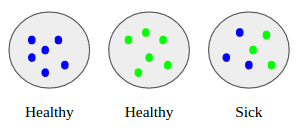
\includegraphics[scale=0.5]{./instance-labels.png}
\caption{This diagram illustrates why static instance labels are not sufficient for phenotype prediction. A patient with 6 of the blue microbe or 6 of the green microbe may be healthy, while a patient with 3 of each is sick. Static instance labels cannot capture this relationship. This is also explained by Amores in his MIL taxonomy \cite{amores13}.} \label{instance-labels}
\end{figure}

\begin{figure}[h]
\centering
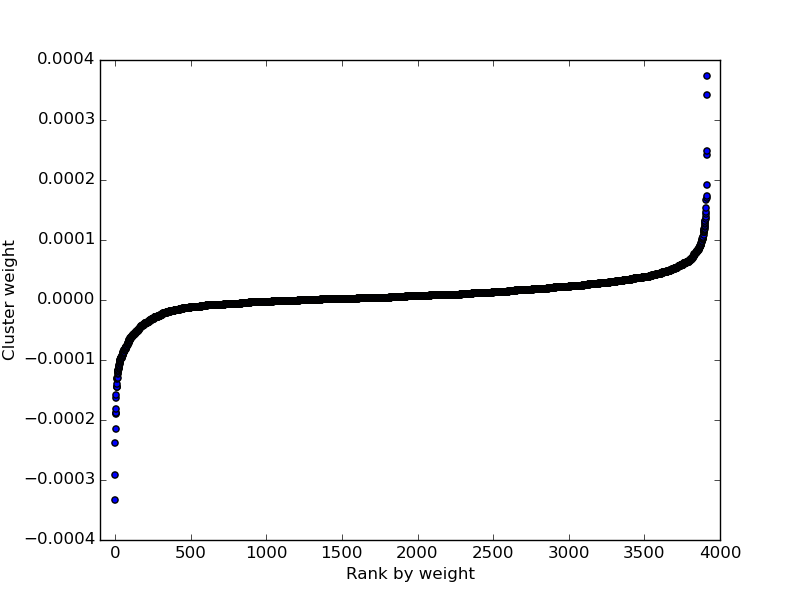
\includegraphics[scale=0.4]{./instance-scatter.png}
\caption{This diagram illustrates the distribution of the instance weights assigned by CAMIL H-BoW. The Y-Axis shows the weights, while the X-Axis shows the ranking of the clusters by weight. Clearly, there are a relatively small number of clusters that have disproportionately large weights or small weights, while the vast majority of the 3918 clusters have weights close to 0.} \label{instance-scatter}
\end{figure}

One of the benefits of using Multiple Instance Learning methods is that we can attempt to discover instance ``labels". In fact, we did not attempt to apply static, unchanging labels to individual reads or clusters, since organisms are affected by their interactions with each other. For instance, a patient with X amount of microbe A or X amount of microbe B may be healthy, but with X/2 amount of microbe A and X/2 amount of microbe B they may be sick. This simple example is illustrated in Figure \ref{instance-labels}.

However, we can infer from the SVM decision boundary which clusters appear to be most relevant to the disease diagnosis. Since feature vectors are multiplied by the weight vector of the decision boundary to determine the label of the patient, we can assume that clusters with the highest weights in the weight vector are most relevant to the disease diagnosis. For instance, if the \emph{i}th scalar in the weight vector is has the highest value of any of the weights, then cluster \emph{i} is likely to play a major role in the disease pathology. Similarly, the most negative weights in the weight vector indicate clusters whose presence in a patient indicates that they likely do not have the disease. Because the data is metagenomic, the clusters represent both phylogenetic and functional similarity, so identifying the most relevant clusters can help discover more about the pathology of the disease. For Type 2 Diabetes, which is a complex phenotype and a disease that is both common and deadly, this is potentially quite valuable.

In the original MGWAS paper, the authors identify 50 important gene markers with mRMR that are used for their classifier. Conversely, CAMIL uses all of the data to train and test the classifier, resulting in 3918 clusters, and subsequently identifies significant clusters based on the classification results. Figure \ref{instance-scatter} is a visual display of the cluster weights determined by CAMIL, using the 344 patient training set and 23 patient test set. Clearly, there are a few clusters with disproportionately high or low weights, while most clusters have weights near 0. Concretely, the lowest cluster weight is -0.000333, the highest is 0.000374, the mean is 0.000008, and the median is 0.000006. Intuitively, this appears to make sense, as there should be a relatively small number of key clusters whose presence is actually indicative of type 2 diabetes, while most other clusters are not particularly relevant in this case and whose weights are just noise. Thus, the weights obtained by this method appear to be plausible. In contrast, the labels obtained by GICF were barely differentiated from each other at all.

\section{Conclusion}
%Conclusion

We have demonstrated an effective and efficient computational pipeline for classifying patient phenotype based on metagenomic data. We have demonstrated that even relatively simple de novo assembly and clustering methods, when used within this pipeline, lead to significantly better performance results than the standard classifier used in the original Metagenome-Wide Association Study. We have shown how to infer the most important OTUs in the disease pathology by using the SVM decision boundary and discussed the clinical importance of this ability. More generally, we have shown the effectiveness of Multiple Instance Learning methods within metagenomics and phenotype prediction, particularly Distance-based Bag of Words methods. Future work could revolve around improving individual parts of the pipeline, such as better assembly and clustering methods, application of different multiple instance learning methods (other than D-BoW), and further attempts to generate more specific instance level information and validate that information against clinical understanding of the diseases.



% conference papers do not normally have an appendix


% use section* for acknowledgement
\section*{Acknowledgment}

The authors would like to extend our 
gratitude towards the Office of Research 
Computing at George Mason University. 
%








% trigger a \newpage just before the given reference
% number - used to balance the columns on the last page
% adjust value as needed - may need to be readjusted if
% the document is modified later
%\IEEEtriggeratref{8}
% The "triggered" command can be changed if desired:
%\IEEEtriggercmd{\enlargethispage{-5in}}

% references section

% can use a bibliography generated by BibTeX as a .bbl file
% BibTeX documentation can be easily obtained at:
% http://www.ctan.org/tex-archive/biblio/bibtex/contrib/doc/
% The IEEEtran BibTeX style support page is at:
% http://www.michaelshell.org/tex/ieeetran/bibtex/
%\bibliographystyle{IEEEtran}
% argument is your BibTeX string definitions and bibliography database(s)
%\bibliography{IEEEabrv,../bib/paper}
%
% <OR> manually copy in the resultant .bbl file
% set second argument of \begin to the number of references
% (used to reserve space for the reference number labels box)

\bibliographystyle{IEEEtran}
% argument is your BibTeX string definitions and bibliography database(s)
\bibliography{./bib/HadoopClustering,./bib/all,./bib/RangwalaRefs,./bib/Rangwala_CV,./bib/anveshi,./bib/disease_state_classifier,./bib/hmp,./bib/lsh,./bib/mgenomics}

%\begin{comment}
%\begin{thebibliography}{1}

%\bibitem{IEEEhowto:kopka}
%H.~Kopka and P.~W. Daly, \emph{A Guide to \LaTeX}, 3rd~ed.\hskip 1em plus
%  0.5em minus 0.4em\relax Harlow, England: Addison-Wesley, 1999.
  
%\bibitem{Goutte}
%C. Goutte and E.Gaussier, \emph{A Probabilistic Interpretation of Precision, Recall and F-score, with Implication for Evaluation}.\hskip 1em plus
%  0.5em minus 0.4em\relax Available at \texttt{http://www.xrce.xerox.com/content/download/16594/118473/file/xrce\_{}eval.pdf}

%\bibitem{ORC}
%\emph{On-Campus Research Computing}.\hskip 1em plus
%  0.5em minus 0.4em\relax Available at \texttt{http://orc.gmu.edu/research-computing/argo-cluster/argo-hardware-specs/}
  
%\bibitem{Joachims08}
%T. Joachims, \emph{SVMlight Support Vector Machine}, 6.02 ed.\hskip 1em plus
%  0.5em minus 0.4em\relax 2008, Available at \texttt{http://svmlight.joachims.org/}

%\bibitem{Wood14}
%D. Wood and S. Salzberg, \emph{Kraken: ultrafast metagenomic sequence classification using exact alignments}.\hskip 1em plus
%  0.5em minus 0.4em\relax 2014, Available at \texttt{http://genomebiology.com/2014/15/3/R46}
  
%\bibitem{Kraken}
%\emph{Kraken Taxonomic Sequence Classification System Operating Manual}, 0.10.5 ed.\hskip 1em plus
%  0.5em minus 0.4em\relax Available at \texttt{https://ccb.jhu.edu/software/kraken/MANUAL.html}

%\bibitem{Edgar10}
%R. Edgar, \emph{Search and Clustering Orders of Magnitude Faster than BLAST}.\hskip 1em plus
%  0.5em minus 0.4em\relax Bioinformatics (2010), 2460--2461. 
  
%\end{thebibliography}

%\end{comment}


% that's all folks
\end{document}


